\subsection{Provenance Data Model serialization}\label{sec:serialisations}


\subsubsection{Serialization of provenance information}

There are two possible families of ProvenanceDM metadata serializations, examples for these can be found here, in the use cases section (\ref{sec:usecases-implementations}), the implementation note \citep[]{std:ProvenanceImplementationNote} and the links therein.

\begin{itemize}

\item PROV-N, PROV-JSON, PROV-XML.
These serialization formats are defined by W3C accompanying their provenance data model. They can be used for the IVOA Provenance Data Model as well.
\begin{itemize}
\item IVOA version: directly serialize all the classes and attributes; pull the description-class attributes into the corresponding main classes or treat them separately (see Section \ref{sec:description-serialization}).
\item W3C compliant versions: Since the W3C model includes the possibility to add additional IVOA or ad hoc attributes to the basic ones in each class, it is possible to produce fully W3C compliant serializations from the IVOA Provenance Data Model. However, a few attributes and class names need to be renamed and ActivityFlow/HadStep need to be reorganized.
\TODO{KR: I guess we need to expand on this?}
\end{itemize}
% They allow the possibility to add additional IVOA or ad hoc attributes to the basic ones in each class. This way the IVOA models can produce W3C compliant serializations. 
% \item Mapping of ProvenanceDM classes onto tables with appropriate relationships. This can allow management by a TAP service (the model mapping is then described with the TAP schema). The serialization will result in a single table according to the query.

 %\TODO{TAP SCHEMA of the ProvenanceDM datamodel: Maybe Mathieu can provide us with a copy of the TAP schema he designed ?}

\item Direct VOTABLE mapping by using an ad hoc mapping based on transcription of PROV-N format: this is called PROV-VOTABLE. Moreover in the future we could also define a VO-DML \citep{std:VODML} version of the mapping.
%The following is an example of provenance metadata in this PROV-VOTABLE format. Objects become tables, their classes are rendered by a utype. Attributes and relationships become FIELDS or PARAMS. The model attribute names also become VOTABLE utypes.

\end{itemize}

These serializations can be produced using the voprov \footnote{\url{https://github.com/sanguillon/voprov}} python module, also see Section~\ref{sec:implementation_voprov}.
Here is an example serialization for an entity being processed by an activity, in PROV-N format:

\begin{verbnobox}[\scriptsize]

document
  prefix ivo <http://www.ivoa.net/documents/rer/ivo/>
  prefix ex <http://www.example.com/provenance/>
  prefix voprov <http://www.ivoa.net/documents/dm/provdm/voprov/>

  entity(ivo://example#Public_NGC6946, [voprov:name="Processed image of NGC 6946"])
  entity(ivo://example#DSS2.143, [voprov:name="Unprocessed image of NGC 6946"])
  activity(ex:Process1, 2017-04-18T17:28:00, 2017-04-19T17:29:00, [voprov:name="Process 1"])
  used(ex:Process1, ivo://example#DSS2.143, -)
  wasGeneratedBy(ivo://example#Public_NGC6946, ex:Process1, 2017-05-05T00:00:00)
endDocument

\end{verbnobox}

This is the corresponding PROV-JSON serialization:

\begin{verbnobox}[\scriptsize]
{
  "prefix": {
    "ivo": "http://www.ivoa.net/documents/rer/ivo/",
    "voprov": "http://www.ivoa.net/documents/dm/provdm/voprov/",
    "ex": "http://www.example.com/provenance/"
  },
  "activity": {
    "ex:Process1": {
      "prov:startTime": "2017-04-18T17:28:00",
      "prov:endTime": "2017-04-19T17:29:00",
      "voprov:name": "Process 1"
    }
  },
  "wasGeneratedBy": {
    "_:id4": {
      "prov:time": "2017-05-05T00:00:00",
      "prov:entity": "ivo://example#Public_NGC6946",
      "prov:activity": "ex:Process1"
    }
  },
  "used": {
    "_:id1": {
      "prov:entity": "ivo://CDS/P/DSS2/POSSII#POSSII.J-DSS2.143",
      "prov:activity": "hips:AlaRGB1"
    }
  }
  "entity": {
    "ivo://example#DSS2.143": {
      "voprov:name": "Unprocessed image of NGC6946"
    },
    "ivo://example#Public_NGC6946": {
      "voprov:name": "Processed image of NGC 6946"
    }
  }
}
\end{verbnobox}

This is the VOTable serialization:

\begin{verbnobox}[\scriptsize]

<?xml version="1.0" encoding="UTF-8"?>
<VOTABLE version="1.2" xmlns="http://www.ivoa.net/xml/VOTable/v1.2" xmlns:ex="http://www.example.com/provenance" xmlns:ivo="http://www.ivoa.net/documents/rer/ivo/" xmlns:voprov="http://www.ivoa.net/documents/dm/provdm/voprov/" xmlns:xsi="http://www.w3.org/2001/XMLSchema-instance" xsi:schemaLocation="http://www.ivoa.net/xml/VOTable/v1.2 http://www.ivoa.net/xml/VOTable/VOTable-1.2.xsd">
  <RESOURCE type="provenance">
    <DESCRIPTION>Provenance VOTable</DESCRIPTION>
    <TABLE name="Usage" utype="voprov:used">
      <FIELD arraysize="*" datatype="char" name="activity" ucd="meta.id" utype="voprov:Usage.activity"/>
      <FIELD arraysize="*" datatype="char" name="entity" ucd="meta.id" utype="voprov:Usage.entity"/>
      <DATA>
        <TABLEDATA>
          <TR>
            <TD>ex:Process1</TD>
            <TD>ivo://example#DSS2.143</TD>
          </TR>
        </TABLEDATA>
      </DATA>
    </TABLE>
    <TABLE name="Generation" utype="voprov:wasGeneratedBy">
      <FIELD arraysize="*" datatype="char" name="entity" ucd="meta.id" utype="voprov:Generation.entity"/>
      <FIELD arraysize="*" datatype="char" name="activity" ucd="meta.id" utype="voprov:Generation.activity"/>
      <DATA>
        <TABLEDATA>
          <TR>
            <TD>ivo://example#Public_NGC6946</TD>
            <TD>ex:Process1</TD>
          </TR>
        </TABLEDATA>
      </DATA>
    </TABLE>
    <TABLE name="Activity" utype="voprov:Activity">
      <FIELD arraysize="*" datatype="char" name="id" ucd="meta.id" utype="voprov:Activity.id"/>
      <FIELD arraysize="*" datatype="char" name="name" ucd="meta.title" utype="voprov:Activity.name"/>
      <FIELD arraysize="*" datatype="char" name="start" ucd="" utype="voprov:Activity.startTime"/>
      <FIELD arraysize="*" datatype="char" name="stop" ucd="" utype="voprov:Activity.endTime"/>
      <DATA>
        <TABLEDATA>
          <TR>
            <TD>ex:Process1</TD>
            <TD>Process 1</TD>
            <TD>2017-04-18 17:28:00</TD>
            <TD>2017-04-19 17:29:00</TD>
          </TR>
        </TABLEDATA>
      </DATA>
    </TABLE>
    <TABLE name="Entity" utype="voprov:Entity">
      <FIELD arraysize="*" datatype="char" name="id" ucd="meta.id" utype="voprov:Entity.id"/>
      <FIELD arraysize="*" datatype="char" name="name" ucd="meta.title" utype="voprov:Entity.name"/>
      <DATA>
        <TABLEDATA>
          <TR>
            <TD>ivo://example#DSS2.143</TD>
            <TD>Unprocessed image of NGC6946</TD>
          </TR>
          <TR>
            <TD>ivo://example#Public_NGC6946</TD>
            <TD>Processed image of NGC 6946</TD>
          </TR>
        </TABLEDATA>
      </DATA>
    </TABLE>
    <INFO name="QUERY_STATUS" value="OK"/>
  </RESOURCE>
</VOTABLE>

\end{verbnobox}

Such serializations can be retrieved through access protocols (see \ref{sec:access_protocols} ) or directly integrated in dataset headers or ``associated metadata'' in order to provide provenance metadata for these datasets. E.g. for FITS files a provenance extension called ``PROVENANCE'' could be added which contains provenance information of the workflow that generated the FITS file in one of the serialisation formats.

%\TODO{Check that this keyword is not already taken.}


% \subsection{Graphic formats} --> moved to implementation section. But may want to
% include a more general section here, mentioning different ways to serialize


\subsubsection{Serialization of description classes}\label{sec:description-serialization}

The ProvenanceDM includes description classes that can exist before any provenance information is recorded. First, the ActivityDescription class gives information on the activity (name, description, doculink...) and the parameters expected as an input. In addition, UsedDescription and WasGeneratedByDescription classes indicate the expected roles of the input and output entities respectively. Finally, The activity may expect specific kinds of entities as inputs or outputs, for which there may be detailed descriptions stored as EntityDescription records.

The serialization of an ActivityDescription, that includes all those description classes, is based on the IVOA DataLink Service Descriptors for service resources \citep{std:Datalink}, and can thus be stored as a VOTable  \citep{std:VOTABLE}. Indeed, a service descriptor points to a service that probably executes an activity using the given input parameters, some of which probably point to entities. One can thus easily translate an ActivityDescription VOTable to a DataLink service descriptor VOTable block, and vice-versa. 

The VOTable contains one resource with attributes type=``meta'' and utype=``voprov:ActivityDescription''. This resource contains PARAM elements to describe the activity and GROUP elements with additional PARAM elements to describe the input parameters (group name=``InputParams''), the input entities (group name=``Used'') and the output entities (group name=``Generated''). 

The standard PARAM elements for an activity resource correspond to the attributes of the ActivityDescription class (see Section~\ref{sec:activity}) and may include an Agent name and email. For the input parameters, each ParameterDescription element is mapped to a PARAM element. The mapping is direct as ParameterDescription is based on PARAM. For the input and output entity groups, each related entity is described with a PARAM block where the name is the role of the entity in the scope of the activity, and the expected value is the entity identifier (utype=``voprov:Entity.id''). It is possible to reference an input parameter using the ref attribute of PARAM, if an input entity is given as an input parameter to the activity (e.g. the name of a file). The xtype attribute of PARAM can be used to provide the content type (MIME type) of the entity.

Here is an example of an ActivityDescription VOTable that describes an activity to create an RGB image from three red, green, blue images:


\begin{verbnobox}[\scriptsize]

<VOTABLE xmlns:xsi="http://www.w3.org/2001/XMLSchema-instance" 
    xmlns="http://www.ivoa.net/xml/VOTable/v1.3" version="1.3" 
    xsi:schemaLocation="http://www.ivoa.net/xml/VOTable/v1.3 
    http://www.ivoa.net/xml/VOTable/v1.3">
  <RESOURCE ID="make_RGB_image" name="make_RGB_image" 
      type="meta" utype="voprov:ActivityDescription">
    <DESCRIPTION>Create an RGB image from 3 images</DESCRIPTION>
    <LINK content-role="doc" href="..."/>
    <PARAM name="label" datatype="char" arraysize="*" 
        value="make_RGB_image" utype="voprov:ActivityDescription.label"/>
    <PARAM name="type" datatype="char" arraysize="*" 
        value="None" utype="voprov:ActivityDescription.type"/>
    <PARAM name="subtype" datatype="char" arraysize="*" 
        value="None" utype="voprov:ActivityDescription.subtype"/>
    <PARAM name="version" datatype="float" 
        value="None" utype="voprov:ActivityDescription.version"/>
    <PARAM name="contact_name" datatype="char" arraysize="*" 
        value="..." utype="voprov:Agent.name"/>
    <PARAM name="contact_email" datatype="char" arraysize="*" 
        value="...@..." utype="voprov:Agent.email"/>
    <GROUP name="InputParams" utype="voprov:Parameter">
      <PARAM ID="RGB" arraysize="*" datatype="char" name="RGB" 
          type="no_query" value="RGB.jpg">
        <DESCRIPTION>RGB image name</DESCRIPTION>
      </PARAM>
      <PARAM ID="order" arraysize="*" datatype="char" name="order" 
          type="no_query" value="RGB">
        <DESCRIPTION>order of the channels</DESCRIPTION>
        <VALUES>
          <OPTION value="RGB"/>
          <OPTION value="RBG"/>
          <OPTION value="GBR"/>
          <OPTION value="GRB"/>
          <OPTION value="BRG"/>
          <OPTION value="BGR"/>
        </VALUES>
      </PARAM>
    </GROUP>
    <GROUP name="Used" utype="voprov:Used">
      <PARAM arraysize="*" datatype="char" name="R" 
          value="R.jpg" utype="voprov:Entity.id" xtype="image/jpeg">
        <DESCRIPTION>Image for red channel</DESCRIPTION>
      </PARAM>
      <PARAM arraysize="*" datatype="char" name="G" 
          value="G.jpg" utype="voprov:Entity.id" xtype="image/jpeg">
        <DESCRIPTION>Image for green channel</DESCRIPTION>
      </PARAM>
      <PARAM arraysize="*" datatype="char" name="B"
          value="B.jpg" utype="voprov:Entity.id" xtype="image/jpeg">
        <DESCRIPTION>Image for blue channel</DESCRIPTION>
      </PARAM>
    </GROUP>
    <GROUP name="Generated" utype="voprov:WasGeneratedBy">
      <PARAM arraysize="*" datatype="char" name="RGB" ref="RGB"
          value="RGB.jpg" utype="voprov:Entity.id"  xtype="image/jpeg">
        <DESCRIPTION>RGB image name</DESCRIPTION>
      </PARAM>
    </GROUP>
  </RESOURCE>
</VOTABLE>

\end{verbnobox}



\subsection{Access protocols}
\label{sec:access_protocols}
We envision two possible access protocols:
\begin{itemize}
\item ProvDAL: retrieve provenance information based on given ID of a data entity or activity.
\item ProvTAP: allows detailed queries for provenance information, discovery of datasets based on e.g. code version.
\end{itemize}

\subsubsection{ProvDAL}
ProvDAL is a simple data access layer interface \citep[see DALI specification of the VO, ][]{std:DALI} that can be implemented by a web service to serve provenance information to a client.
%It follows the basic DALI principles of the VO as detailed in \citep[see][]{std:DALI}.
The client sends GET request to the basic URL endpoint (\texttt{\{provdal-base-url\}}) of a ProvDAL service, providing at least the main parameter {\bf ID}, the (unique, qualified) identifier of an entity (obs\_publisher\_did of an ObsDataSet for example), activity or an agent. This parameter can occur more than once in a request in order to retrieve provenance details for several activities, datasets or agents at the same time. Here are two simple example requests:

\begin{verbatim}
{provdal-base-url}?ID=rave:dr4
{provdal-base-url}?ID=rave:dr4&ID=rave:act_irafReduction
\end{verbatim}
\noindent
Additional parameters can complete the request to refine the query. They are described in the next paragraphs and summarized in Table~\ref{tab:provdal-parameters}.

\begin{table}[h]
\small
\begin{tabulary}{1.0\textwidth}{@{}p{0.17\textwidth}p{0.22\textwidth}p{0.53\textwidth}@{}}
%{llp{0.2\textwidth}p{0.3\textwidth}}
\toprule
\head{Parameter} & \head{Values} & \head{Description}\\\hline
\midrule
\textbf{\urlparam{ID}} & qualified \urlparam{ID} & a valid qualified identifier for an entity, activity or agent (can occur multiple times)\\
\textbf{\urlparam{DEPTH}} & 0,\underline{1},2,..., \urlparam{ALL} &  number of relations to be followed or \texttt{ALL} for everything, independent of the relation type\\
\textbf{\urlparam{FORMAT}} & \urlparam{PROV-N}, \newline\urlparam{\underline{PROV-JSON}}, \newline\urlparam{PROV-XML}, \newline\urlparam{PROV-VOTABLE} & serialisation format of the response\\\hline
\urlparam{DIRECTION} & \urlparam{\underline{BACK}}, \urlparam{FORTH} & \urlparam{BACK} = track the provenance history, \newline\urlparam{FORTH} = explore the results of activities and where entities have been used\\
\urlparam{MEMBERS} & \urlparam{true} or \urlparam{\underline{false}} & if \urlparam{true}, retrieve and track members of collections\\
\urlparam{STEPS} & \urlparam{true} or \urlparam{\underline{false}} & if \urlparam{true}, retrieve and track steps of activityFlows\\
\urlparam{AGENT} & \urlparam{true} or \urlparam{\underline{false}} & if \urlparam{true}, explore all relations for agents, i.e. find out what an agent is responsible for\\
\bottomrule
\end{tabulary}
\caption{ProvDAL request parameters. Options that are \textbf{required} to be implemented by ProvDAL services are marked with bold face. \underline{Default} values are underlined. The parameter names are case-insensitive, but the parameter values are not.}
\label{tab:provdal-parameters}
\end{table}


\paragraph{Response format}
The format of the response can be defined using the FORMAT parameter. Its value is one of the provenance serialization formats: PROV-N, PROV-JSON, PROV-XML, PROV-VOTABLE.

\TODO{Rename FORMAT to RESPONSEFORMAT as in DALI, Section 3.4.3?}

\paragraph{{DEPTH}}
The DEPTH parameter gives the number of relations that shall be tracked along
the provenance history -- independent of the type of relation. Its value is
either 0, a positive integer or ALL. If this parameter is omitted,
the default is 1, which returns all relations and nodes that can be reached
by following 1 relation. If \texttt{DEPTH=ALL} is requested, the server should
return the complete provenance history that the service has stored for the
given entity, activity or agent. 

\TODO{KR: add here: 
Services may restrict the returned data by
redirecting \texttt{DEPTH=ALL} to e.g. \texttt{DEPTH=\{maxdepth\}}, where
\texttt{\{maxdepth\}} is an integer defining the maximum depth number that
the server allows.}

Note that the relations \emph{wasDerivedFrom} and \emph{wasInformedBy} are ``short-cuts''
in a provenance graph. Thus for e.g. \texttt{DEPTH=2} more progenitors of an entity may
be reached via \emph{wasDerivedFrom} relations than via the ``long path'' along the
corresponding \emph{used} and \emph{wasGeneratedBy} relations (see e.g. progenitor entity E1 in
Figure~\ref{fig:provenance-graph-example}).
%Whenever DEPTH is not ALL, the client has to accept that
%the returned part of a provenance graph may not be complete and that nodes may be returned
%which are related to each other but the relations are not shown (yet).
%(because they would only appear if DEPTH is increased.)
(A better solution for the future may be to use 1/2*DEPTH for walking along these short-cut relations, but we don't want to make ProvDAL more complex for now.)

% \noindent
% The format can also be specified via the HTTP accept header, e.g.
% \begin{verbatim}
% wget -d --header="Accept: application/json" \
%    {provdal-base-url}?ID=rave:dr4
% \end{verbatim}
% would return the provenance information in \urlparam{PROV-JSON} format.
% \noindent
% If both \urlparam{FORMAT} and the accept header are used and \urlparam{FORMAT} specifies a format that is incompatible with the HTTP accept header, then the service should return with a HTTP status 406: Not Acceptable.

\paragraph{DIRECTION}
For services which allow tracking the provenance information forward, e.g. in order to check for which activities an entity was used, the optional parameter DIRECTION can be set to FORTH. Its default value is BACK. This only influences the direction in which the used, wasGeneratedBy, wasDerivedFrom and wasInfluencedBy relations are followed. Any other relations are tracked according to the behaviour specified below, independent of the DIRECTION value.

Figure~\ref{fig:provenance-graph-example} shows an example provenance graph with different relations and nodes. Only the relations marked by solid lines are influenced by the DIRECTION parameter. A ProvDAL GET request with \texttt{ID=E6} and \texttt{DEPTH=2} returns only the highlighted nodes and relations (thick lines) by default.

\begin{figure}[h]
\centering
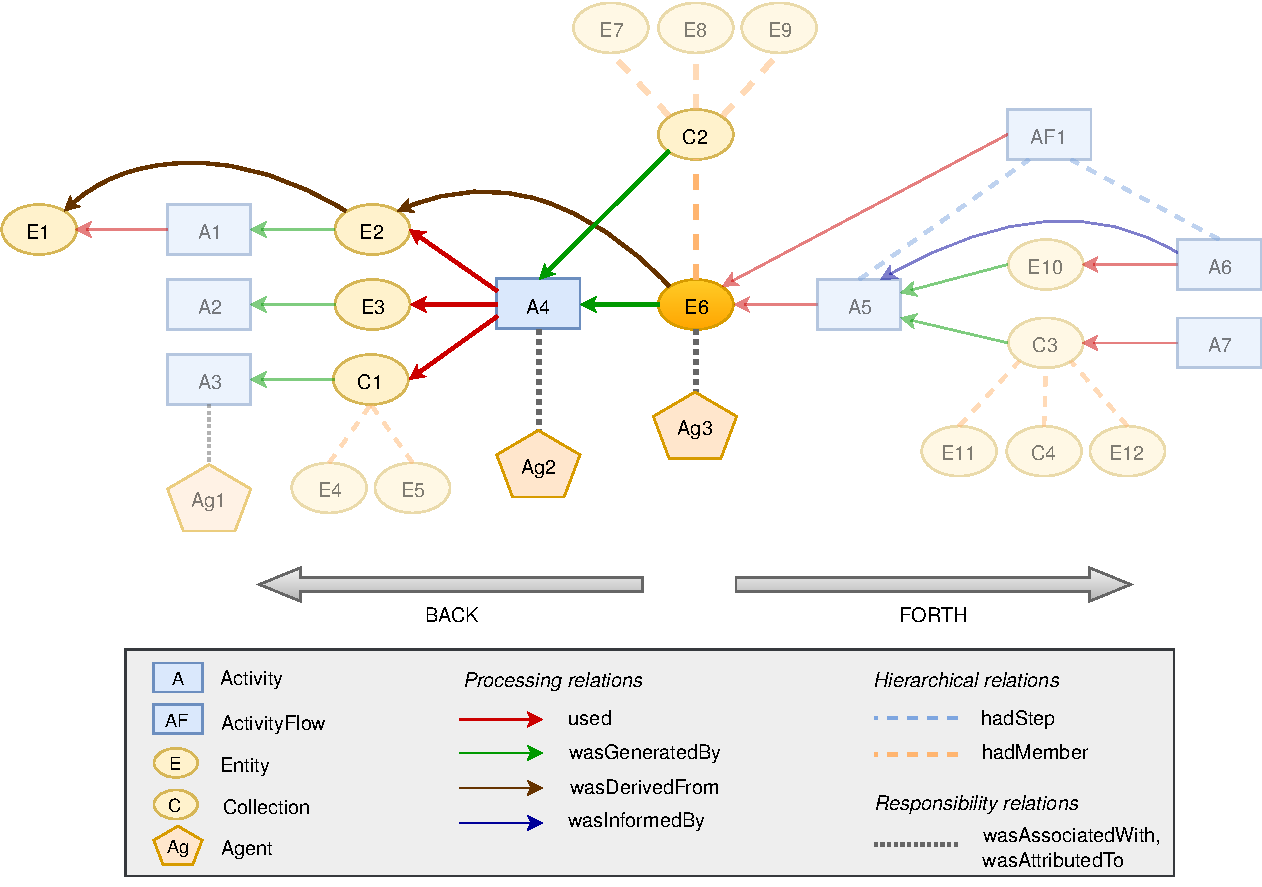
\includegraphics[width=1.0\textwidth]{provenance-graph-example-depth2.pdf}
\caption{An example provenance graph, highlighting the objects and relations returned from a ProvDAL service with \texttt{ID=E6} and \texttt{DEPTH=2}. The BACK and FORTH values for DIRECTION are only important for the processing relations (solid lines). Hierarchial (dashed) and responsibility (dotted) relations are only followed ``upwards'' (to collection/activityFlow) and towards agents by default (unless the optional parameters MEMBERS, STEPS and/or AGENT are set to true.}
\label{fig:provenance-graph-example}
\end{figure}




\paragraph{MEMBERS, STEPS}
The provenance data model defines the hierarchical relations \emph{hadMember} for entity collections and \emph{hadStep} for activityFlows. If a node belongs to a collection or activityFlow, these relations shall be returned as well, independent of the specified tracking direction.
If someone is interested in more details and wants to follow the \emph{members} of an entity collection or the \emph{steps} of an activityFlow, these can be included by setting the optional parameter MEMBERS or STEPS to true, respectively. The default is false. As detailed in DALI, the values 1 and 0 are equivalent to true and false.

\paragraph{AGENT}
By default, it is recommended to stop any further tracking at an agent node, unless an additional optional parameter AGENT is set to true. Note that this means that the request for any agent will always return just the agent node itself and nothing else, unless AGENT=true is used. An example request if one wants to know which entities and activities an agent has influenced could look like this:\\\texttt{\{provdal-base-url\}?ID=org:rave\&AGENT=true\&DEPTH=1}.\\
\texttt{DEPTH=1} is used here in order to avoid following the found entities and activities any further (can be omitted, since this is the default for DEPTH).
\newline
%\comment{Maybe it's better to use DEPTH and DIRECTION instead of FORWARD and BACKWARD. Reason: if a service just implements the backward direction, then it's weird to call something ``backward'' if there is no ``forward'' as well. DEPTH is also a commonly used word when refering to graphs and numbers of relations.}



A ProvDAL service MUST implement the parameters ID, DEPTH and FORMAT; the remaining parameters are optional.
If a service does not implement the optional parameters, but they appear in the request, then the service should return with an error.
Please note that according to the DALI specification \citep{std:DALI}, the parameter names are case-insensitive, but the parameter values are not. E.g. \texttt{direcion=FORTH} is allowed, but \texttt{DIRECTION=forth} may not work.


\subsubsection{ProvDAL example use cases}
We provide here a few example use cases for ProvDAL in order to show its usefulness in exploring the provenance
of astronomical datasets, processes or the people and projects involved in producing/performing them.

\begin{itemize}
\item The RAVE DR4 release contains a main table with stellar properties for each observation of a star. Given the RAVE observation ID, retrieve the processing steps
for this specific observation result:

	\begin{verbatim}
	{provdal-base-url}?ID=rave:20121220_0752m38_089&DEPTH=ALL
	\end{verbatim}

The result will not only contain the processing steps (activities), but also entities and agents. The important information can be filtered out by a client application (e.g. use voprov Python package). If a W3C tool shall be used, one needs to transform the response into a W3C compliant serialisation (e.g. for loading the result to ProvStore\footnote{https://provenance.ecs.soton.ac.uk/store/} for further processing).

\item Get the direct progenitor of an entity:
	\begin{verbatim}
	{provdal-base-url}?ID=rave:20121220_0752m38_089&DEPTH=1
	\end{verbatim}
	If this request only returns a collection and not any ``backwards'' information about progenitors, then
	one needs to track the collection further, i.e. repeat the request for the collection entity.

\item Get all datasets that were derived from a specific data file in the CTA pipeline:
	\begin{verbatim}
	{provdal-base-url}?ID=cta:df1&DEPTH=ALL&DIRECTION=FORTH
	\end{verbatim}
	By using \texttt{DIRECTION=FORTH} we can track the dataset and where it was used forward.

\item Find all people that were involved in processing a dataset along with their contact data (if available), so that one can ask them for further information.
	\begin{verbatim}
	{provdal-base-url}?ID=ex:e1&DEPTH=ALL
	\end{verbatim}
 	The ProvDAL request is basically the same as in the first example. From the results the agents need to be filtered.
 	Since the response contains the nodes and relations including all their properties, the contact details for the agents are included as well (if they are stored with the service).

\item Retrieve a VOTABLE serialisation of the provenance for an image from a data collection.
	\begin{verbatim}
	{provdal-base-url}?ID=myproject:img1&DEPTH=ALL&FORMAT=PROV-VOTABLE
	\end{verbatim}
	We use the FORMAT keyword here to retrieve a VOTABLE.
\end{itemize}

ProvDAL is meant to be used to retrieve parts of a provenance graph from a provenance web service. It cannot be used to retrieve information based on specific properties, e.g. the creationTime of an entity or a parameter value for an activity. For such cases, a ProvTAP service can be used (see next section).


\TODO{Add paragraph on VOSI-endpoints? (DALI service!)}



\subsubsection{ProvTAP}
ProvTAP is a TAP service implementing the ProvenanceDM data model. The data model mapping is included in the TAP schema. The mapping of ProvenanceDM classes and attributes onto tables and columns of the schema with the appropriate relationships, datatypes, units, utypes and ucds is done similarly to the PROV-VOTABLE serialization. The query response will result in a single table according to the query.
This single table is joining information coming from one or several ``provenance'' tables available in the database.

A special case is considered where ProvenanceDM and ObsCore are both implemented in the same TAP service and queried together. The TAP response is then providing an Obscore table with a ProvenanceDM extension. We can imagine that in the future this could be hard-coded and registered as an ObsProvTAP service.


\TODO{We need more details here! Output of TAP service is NOT a PROV-VOTABLE by default!}

%\TODO{Do we need combined query possibilities, i.e. ask for ObsCore-fields and Provenance fields in one query? Or rather use a 2-step-process, decoupling them from each other?}


%\TODO{Also look at PROV-AQ from the W3C.}

\subsubsection{VOSI availability and capabilities}
According to the DALI specification for VO services \citep{std:DALI}, a provenance service implementing ProvDAL and/or ProvTAP must provide a VOSI availability interface as well as a capabilities interface with entries for ProvDAL and/or ProvTAP. The \texttt{standardId}s for these provenance interfaces are:

\begin{verbatim}
ivo://ivoa.net/std/ProvenanceDM#ProvDAL-1.0
ivo://ivoa.net/std/ProvenanceDM#ProvTAP-1.0
\end{verbatim}

For ProvTAP, the VOSI tables interface also needs to be provided.

